\documentclass[border=5mm]{standalone}
\usepackage{tikz}
\tikzset{real edge/.style={solid,very thick, -latex}}

\begin{document}
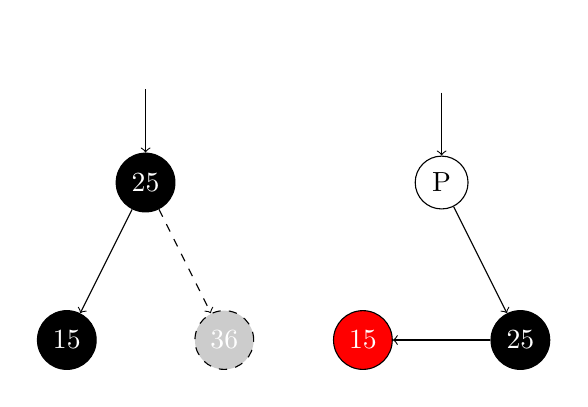
\begin{tikzpicture}
    \matrix[row sep=1cm, column sep=1cm] {
        \node[circle] (0) at (0, 1.5) {\textcolor{white}{0}};
        \node[draw, fill=black, circle] (25) at (0, 0) {\textcolor{white}{25}};
        \node[draw, fill=black, circle] (15) at (-1, -2) {\textcolor{white}{15}};
        \node[draw, dashed, fill=black!20, circle] (36) at (1, -2) {\textcolor{white}{36}};

        \draw[->] (0) -- (25);
        \draw[->] (25) -- (15);
        \draw[dashed, ->] (25) -- (36);
         &
        \node[circle] (-1) at (0, 1.5) {\textcolor{white}{-1}};
        \node[draw, circle] (0) at (0, 0) {\textcolor{black}{P}};
        \node[draw, fill=red, circle] (15) at (-1, -2) {\textcolor{white}{15}};
        \node[draw, fill=black, circle] (25) at (1, -2) {\textcolor{white}{25}};

        \draw[->] (-1) -- (0);
        \draw[->] (0) -- (25);
        \draw[->] (25) -- (15);

        \\
    };
\end{tikzpicture}
\end{document}
